% Author: Izaak Neutelings (November 2021)
% Inspiration: Kyle Cormier
\documentclass[border=3pt,tikz]{standalone}
\usepackage{physics}
\usepackage{tikz}
\usepackage{tikz-3dplot}
%\usepackage[outline]{contour} % glow around text
\usepackage{xcolor}

\colorlet{myred}{red!70!black}
\colorlet{myblue}{blue!80!black}
\colorlet{mygreen}{green!50!black}
\colorlet{myorange}{orange!80!black}
\colorlet{mydarkred}{red!40!black}
\colorlet{mydarkblue}{blue!40!black}
\colorlet{mydarkgreen}{green!30!black}
\colorlet{mydarkorange}{orange!60!black}
\tikzset{>=latex} % for LaTeX arrow head
\tikzstyle{vector}=[->,mygreen,thick,line cap=round]
\tikzstyle{dot}=[circle,inner sep=0.8,outer sep=0.02]
%\contourlength{1.3pt}
\newcommand*{\vv}[1]{\vec{\mkern0mu#1}} % aligned vector arrow
\def\tick#1{\draw[thick] (#1) --++ (0,0.08);}
\def\point#1#2{
  \fill (#1) circle(0.02);
  \draw[line width=0.65] (#1)++(0,#2) --++ (0,-2*#2);
  \draw[line width=0.65] (#1)++(-0.03,#2) --++ (0.06,0);
  \draw[line width=0.65] (#1)++(-0.03,-#2) --++ (0.06,0);
}

\begin{document}


% HISTOGRAM - 2 bins
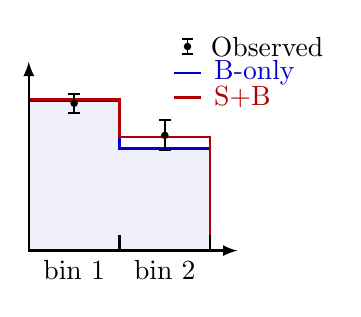
\begin{tikzpicture}[scale=2.4]
  \coordinate (O) at (0,0,0);
  \def\w{0.48}
  
  % HISTOGRAMS
  \draw[thick,myblue,fill=myblue!6]
    (0,0) -- (0,0.79) -| (\w,0.54) -| (2*\w,0) -- cycle;
  \draw[thick,myred] (0,0.80) -|++ (\w,-0.20) -| (2*\w,0);
  \point{0.5*\w,0.78}{0.05}
  \point{1.5*\w,0.61}{0.08}
  
  % AXES
  \draw[<->,thick] (2.3*\w,0) -- (O) -- (0,1);
  \node[below=0] at (0.5*\w,0) {bin 1};
  \node[below=0] at (1.5*\w,0) {bin 2};
  \tick{\w,0}
  \tick{2*\w,0}
  
  % LEGEND
  \point{1.75*\w,1.08}{0.04}
  \node[right] at (1.9*\w,1.08) {Observed};
  \draw[thick,myblue] (1.6*\w,0.94) --++ (0.3*\w,0) node[right=1] {B-only};
  \draw[thick,myred] (1.6*\w,0.81) --++ (0.3*\w,0) node[right=1] {S+B};
  
\end{tikzpicture}


% HISTOGRAM - 2 bins, systematic variation
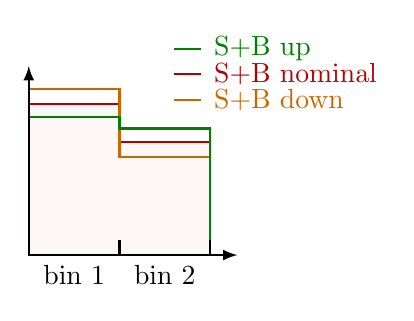
\begin{tikzpicture}[scale=2.4]
  \coordinate (O) at (0,0,0);
  \def\w{0.48}
  
  % HISTOGRAMS
  \draw[thick,myred,fill=myred!3]
    (0,0) -- (0,0.80) -| (\w,0.60) -| (2*\w,0) -- cycle;
  \draw[thick,myorange] % down variation
    (0,0.88) -| (\w,0.52) -| (2*\w,0);
  \draw[thick,mygreen] % up variation
    (0,0.73) -| (\w,0.67) -| (2*\w,0);
  
  % AXES
  \draw[<->,thick] (2.3*\w,0) -- (O) -- (0,1);
  \node[below=0] at (0.5*\w,0) {bin 1};
  \node[below=0] at (1.5*\w,0) {bin 2};
  \tick{\w,0}
  \tick{2*\w,0}
  
  % LEGEND
  \draw[thick,mygreen] (1.6*\w,1.09) --++ (0.3*\w,0) node[right=1] {S+B up};
  \draw[thick,myred] (1.6*\w,0.96) --++ (0.3*\w,0) node[right=1] {S+B nominal};
  \draw[thick,myorange] (1.6*\w,0.82) --++ (0.3*\w,0) node[right=1] {S+B down};
  
\end{tikzpicture}


% HISTOGRAM - 3 bins
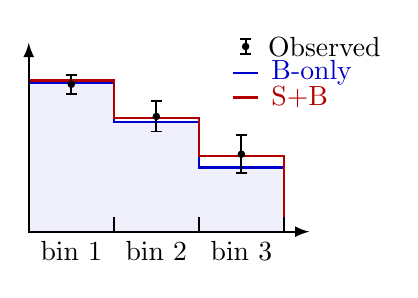
\begin{tikzpicture}[scale=2.4]
  \coordinate (O) at (0,0,0);
  \def\w{0.45}
  
  % HISTOGRAMS
  \draw[thick,myblue,fill=myblue!6]
    (0,0) -- (0,0.79) -| (\w,0.58) -| (2*\w,0.34) -| (3*\w,0) -- cycle;
  \draw[thick,myred] (0,0.80) -| (\w,0.60) -| (2*\w,0.40) -| (3*\w,0);
  \point{0.5*\w,0.78}{0.05}
  \point{1.5*\w,0.61}{0.08}
  \point{2.5*\w,0.41}{0.10}
  
  % AXES
  \draw[<->,thick] (3.3*\w,0) -- (O) -- (0,1);
  \node[below=0] at (0.5*\w,0) {bin 1};
  \node[below=0] at (1.5*\w,0) {bin 2};
  \node[below=0] at (2.5*\w,0) {bin 3};
  \tick{\w,0}
  \tick{2*\w,0}
  \tick{3*\w,0}
  
  % LEGEND
  \point{2.55*\w,0.98}{0.04}
  \node[right] at (2.7*\w,0.98) {Observed};
  \draw[thick,myblue] (2.4*\w,0.84) --++ (0.3*\w,0) node[right=1] {B-only};
  \draw[thick,myred] (2.4*\w,0.71) --++ (0.3*\w,0) node[right=1] {S+B};
  
\end{tikzpicture}


% 2D AXIS
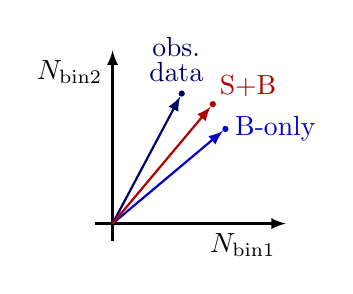
\begin{tikzpicture}[scale=2.2]
  \coordinate (O) at (0,0,0);
  \coordinate (D) at (62:0.85); % observed data
  \coordinate (B) at (40:0.85); % B-only
  \coordinate (S) at (50:0.90); % S+B
  
  % AXES
  \draw[thick,->] (-0.1,0) -- (1,0) node[below left=0]{$N_\text{bin1}$};
  \draw[thick,->] (0,-0.1) -- (0,1) node[below left=0]{$N_\text{bin2}$};
  
  % POINTS
  \node[dot,fill=mydarkblue] (D') at (D) {};
  \node[dot,fill=myblue] (B') at (B) {};
  \node[dot,fill=myred] (S') at (S) {};
  
  % VECTORS
  \draw[vector,mydarkblue] (O)  -- (D');
  \draw[vector,myblue] (O)  -- (B');
  \draw[vector,myred] (O)  -- (S');
  
  % LABELS
  \node[mydarkblue,left=2,above=1,align=center] at (D) {obs.\\[-3]data};
  \node[myblue,right=0] at (B) {B-only};
  \node[myred,above right=-1] at (S) {S+B};
  
\end{tikzpicture}


% 2D AXIS - systematic variation
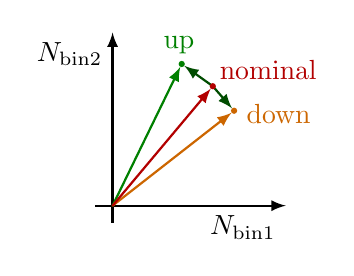
\begin{tikzpicture}[scale=2.2]
  \coordinate (O) at (0,0,0);
  \coordinate (D) at (38:0.89); % up
  \coordinate (N) at (50:0.90); % nominal
  \coordinate (U) at (64:0.91); % down
  
  % AXES
  \draw[thick,->] (-0.1,0) -- (1,0) node[below left=0]{$N_\text{bin1}$};
  \draw[thick,->] (0,-0.1) -- (0,1) node[below left=0]{$N_\text{bin2}$};
  
  % POINTS
  \node[dot,fill=myorange] (D') at (D) {};
  \node[dot,fill=mygreen] (U') at (U) {};
  \draw[vector,mydarkgreen] (N) -- (U');
  \draw[vector,mydarkgreen] (N) -- (D');
  \node[dot,fill=myred] (N') at (N) {};
  
  % VECTORS
  \draw[vector,myorange] (O)  -- (D');
  \draw[vector,mygreen] (O)  -- (U');
  \draw[vector,myred] (O)  -- (N');
  
  % LABELS
  \node[myorange,below=1,right=1] at (D) {down};
  \node[myred,above right=-1] at (N) {nominal};
  \node[mygreen,left=1,above=0] at (U) {up};
  
\end{tikzpicture}


% 3D AXIS
\tdplotsetmaincoords{67}{115}
\begin{tikzpicture}[scale=2.6,tdplot_main_coords]
  \def\w{1.5} % plane width
  \coordinate (O) at (0,0,0);
  \coordinate (D) at (0.9,0.8,1.1); % observed data
  \coordinate (B) at (1.0,1.1,0.9); % B-only
  \coordinate (S) at (0.7,1.0,1.0); % S+B
  
  % AXES
  \draw[thick,->] (O) -- (1,0,0) node[below left=-2]{$N_\text{bin1}$};
  \draw[thick,->] (O) -- (0,1,0) node[right=-1]{$N_\text{bin2}$};
  \draw[thick,->] (O) -- (0,0,1) node[above=-1]{$N_\text{bin3}$};
  
  % VECTORS
  \node[dot] (B') at (B) {};
  \node[dot] (S') at (S) {};
  \node[dot] (D') at (D) {};
  \draw[vector,mydarkblue] (O)  -- (D');
  \draw[vector,myblue] (O)  -- (B');
  \draw[vector,myred] (O)  -- (S');
  
  % PLANE
  %\fill[mydarkblue,opacity=0.2] (D) -- (B) -- (S) -- cycle;
  \fill[myblue!8,opacity=0.6]
    (D)++(-0.4*\w,-0.2,0.2) --++ (\w,0,0) --++ (0,0.85,-0.6) --++ (-\w,0,0) -- cycle;
  
  % VECTORS in plane
  \draw[vector] (D) -- (B');
  \draw[vector] (D) -- (S');
  
  % POINTS
  \node[dot,fill=mydarkblue] at (D) {};
  \node[dot,fill=myblue] at (B) {};
  \node[dot,fill=myred] at (S) {};
  
  % LABELS
  \node[mydarkblue,above=0,align=center] at (D) {obs.\\[-3]data};
  \node[myblue,below right=-2] at (B) {B-only};
  \node[myred,right=0] at (S) {S+B};
  
\end{tikzpicture}


% ORTHONORMAL BASIS
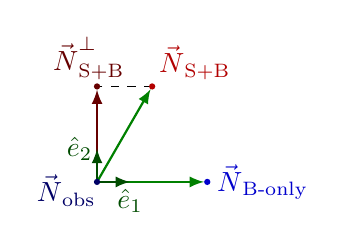
\begin{tikzpicture}[scale=1.4]
  \def\ang{60}
  \def\u{0.3} % unit length
  \coordinate (O) at (0,0,0);
  \coordinate (B) at (1,0); % B-only
  \coordinate (S) at (\ang:1); % S+B
  \coordinate (P) at (0,{sin(\ang)}); % S+B projection
  
  % POINTS
  \draw[dashed] (S) -- (P);
  \node[dot,fill=myblue] (B') at (B) {};
  \node[dot,fill=myred] (S') at (S) {};
  \node[dot,fill=mydarkred] (P') at (P) {};
  
  % VECTORS
  \draw[vector] (O)  -- (B');
  \draw[vector] (O)  -- (S');
  \draw[vector,mydarkred] (O)  -- (P');
  \draw[vector,mydarkgreen] (O)  -- (\u,0) node[below=-1] {$\hat{e}_1$};
  \draw[vector,mydarkgreen] (O)  -- (0,\u) node[left=-2] {$\hat{e}_2$};
  \node[dot,fill=mydarkblue] at (O) {};
  
  % LABELS
  \node[mydarkblue,above=3,below left=-3] at (O) {$\vv{N}_\text{obs}$};
  \node[myblue,right=0] at (B) {$\vv{N}_\text{B-only}$};
  \node[myred,above right=-1] at (S) {$\vv{N}_\text{S+B}$};
  \node[mydarkred,left=3,above=-1] at (P) {$\vv{N}_\text{S+B}^\perp$};
  
\end{tikzpicture}


\end{document}